\documentclass[a4paper]{article}

\setlength{\parindent}{0pt}
\setlength{\parskip}{1em}

\pagestyle{headings}

\usepackage{amssymb}
\usepackage{amsmath}
\usepackage{amsthm}
\usepackage{mathtools}
\usepackage{graphicx}
\usepackage{hyperref}
\usepackage{color}
\usepackage{microtype}
\usepackage{tikz}
\usepackage{pgfplots}
\usepackage{pgfplotstable}

\newcommand{\N}{\mathbb{N}}
\newcommand{\Q}{\mathbb{Q}}
\newcommand{\Z}{\mathbb{Z}}
\newcommand{\R}{\mathbb{R}}
\newcommand{\C}{\mathbb{C}}
\newcommand{\D}{\mathcal{D}}
\renewcommand{\S}{\mathcal{S}}
\renewcommand{\P}{\mathbb{P}}
\newcommand{\F}{\mathbb{F}}
\newcommand{\E}{\mathbb{E}}
\newcommand{\bra}{\langle}
\newcommand{\ket}{\rangle}


\graphicspath{{Image/}}

\hypersetup{
    colorlinks=true,
    linktoc=all,
    linkcolor=blue
}

\theoremstyle{definition}
\newtheorem*{axiom}{Axiom}
\newtheorem*{claim}{Claim}
\newtheorem*{conv}{Convention}
\newtheorem*{coro}{Corollary}
\newtheorem*{defi}{Definition}
\newtheorem*{eg}{Example}
\newtheorem*{lemma}{Lemma}
\newtheorem*{notation}{Notation}
\newtheorem*{prob}{Problem}
\newtheorem*{post}{Postulate}
\newtheorem*{prop}{Proposition}
\newtheorem*{rem}{Remark}
\newtheorem*{thm}{Theorem}

\DeclareMathOperator{\vdiv}{div}
\DeclareMathOperator{\grad}{grad}
\DeclareMathOperator{\curl}{curl}
\DeclareMathOperator{\Ann}{Ann}
\DeclareMathOperator{\Fit}{Fit}
\DeclareMathOperator{\Diag}{Diag}
\DeclareMathOperator{\tr}{tr}
\DeclareMathOperator{\im}{im}
\DeclareMathOperator{\Mat}{Mat}
\DeclareMathOperator{\Log}{Log}
\DeclareMathOperator{\Isom}{Isom}
\DeclareMathOperator{\Mesh}{Mesh}
\DeclareMathOperator{\Sym}{Sym}
\DeclareMathOperator{\Aut}{Aut}
\DeclareMathOperator{\cosech}{cosech}
\DeclareMathOperator{\Card}{Card}
\DeclareMathOperator{\Gal}{Gal}


\setcounter{section}{-1}

\begin{document}

\title{Applied Probability}

\maketitle

\newpage

\tableofcontents

\newpage

\section{Miscellaneous}

Some speech

Google lecture's name to find his homepage and example sheets or probably some notice of a change of room

\newpage

\section{Poisson process}

Suppose we have a Geiger counter. We model the "click process" as a family $\{N(t) : t \geq 0\}$, where $N(t)$ denotes the total number of ticks up to time $t$. Now note that $N(t) \in \{0,1,...\}$, $N(s) \leq N(t)$ if $s \leq t$, $N$ increases by unit jumps, and $N(0) = 0$. We also assert that $N$ is right-continuous, i.e. $\lim_{x \to t^+} N(x) = N(t)$.

\begin{defi} (infinitesimal definition)\\
A \emph{Poisson process} with intensity $\lambda$ is a process $N=(N(t):t \geq 0)$ which takes values in $S = \{0,1,2,...\}$, s.t.:\\
(a) $N(0) = 0$, $N(s) \leq N(t)$ if $s \leq t$;\\
(b) 
\begin{equation*}
\begin{aligned}
\P(N(t+h)=n+m | N(t) = n) = \left\{\begin{array}{ll}
\lambda h + o(h) & m=1\\
o(h) & m>1\\
1-\lambda h & m=0
\end{array}
\right.
\end{aligned}
\end{equation*}
Recall that $g(h) = o(h)$ means that $\frac{g(h)}{h} \to 0$ as $h \to 0$;\\
(c) if $s<t$, then $N(t)-N(s)$ is independent of all arrivals prior to $s$.
\end{defi}

\begin{thm}
$N(t)$ has the Poisson distribution with parameter $\lambda t$.
\begin{proof}
Study $N(t+h)$ given $N(t)$. We have 
\begin{equation*}
\begin{aligned}
\P(N(t+h) =j) &= \sum_{i\leq j} \P(N(t+h) \\
&= j|N(t) = i) \P(N(t) = i) \\
&= (1-\lambda h) \P(N(t) = j) + \lambda h \P(N(t) = h-1) + o(h)
\end{aligned}
\end{equation*}
So
\begin{equation*}
\begin{aligned}
\frac{\P(N(t+h)=j) - \P(N(t) = j)}{h} = -\lambda \P(N(t) = j) + \lambda \P (N(t) = j-1) + \frac{o(h)}{h}
\end{aligned}
\end{equation*}
write $p_n(t) = \P(N(t) = n)$, then let $h \to 0^+$ we get
\begin{equation*}
\begin{aligned}
p'_j(t) &= -\lambda p_j(t) + \lambda p_{j-1}(t) & j \geq 1\\
p'_0(t) &= -\lambda p_0(t) &
\end{aligned}
\end{equation*}
with boundary condition $p_0(0) = 1$.\\
We solve $p_0$ to get $p_0(t) = e^{-\lambda(t)}$. Then we can use this to inductively solve $p_1,p_2,...$ to get the desired result.
\end{proof}
\end{thm}

An alternative derivation from the differential equations:\\
Let $G(s,t) = \sum_j s^j p_j(t)$. Now we take the set of differential equation, multiplying each one by $s^j$, then we get
\begin{equation*}
\begin{aligned}
\frac{\partial G}{\partial t} = \lambda (s-1) G
\end{aligned}
\end{equation*}
Then we have $$G(s,t) = A(s) e^{\lambda (s-1) t}$$ We also have $G(s,0)=1$ so we should be able to plug in a suitable value of $s$ to get the desired result (I probably missed that).

\begin{defi}(Holding/interarrival times)
In a poisson process (pp) with parameter $\lambda$, let $N(t)$ denote the total number of "clicks". Define the arrival times $T_0 = 0$, $T_n = \inf \{t \geq 0: N(t) = n\}$, i.e. the first time $t$ that $N$ reaches $n$ (note right continuity of $N$). We also define the interarrival times $X_n = T_n - T_{n-1}$.
\end{defi}

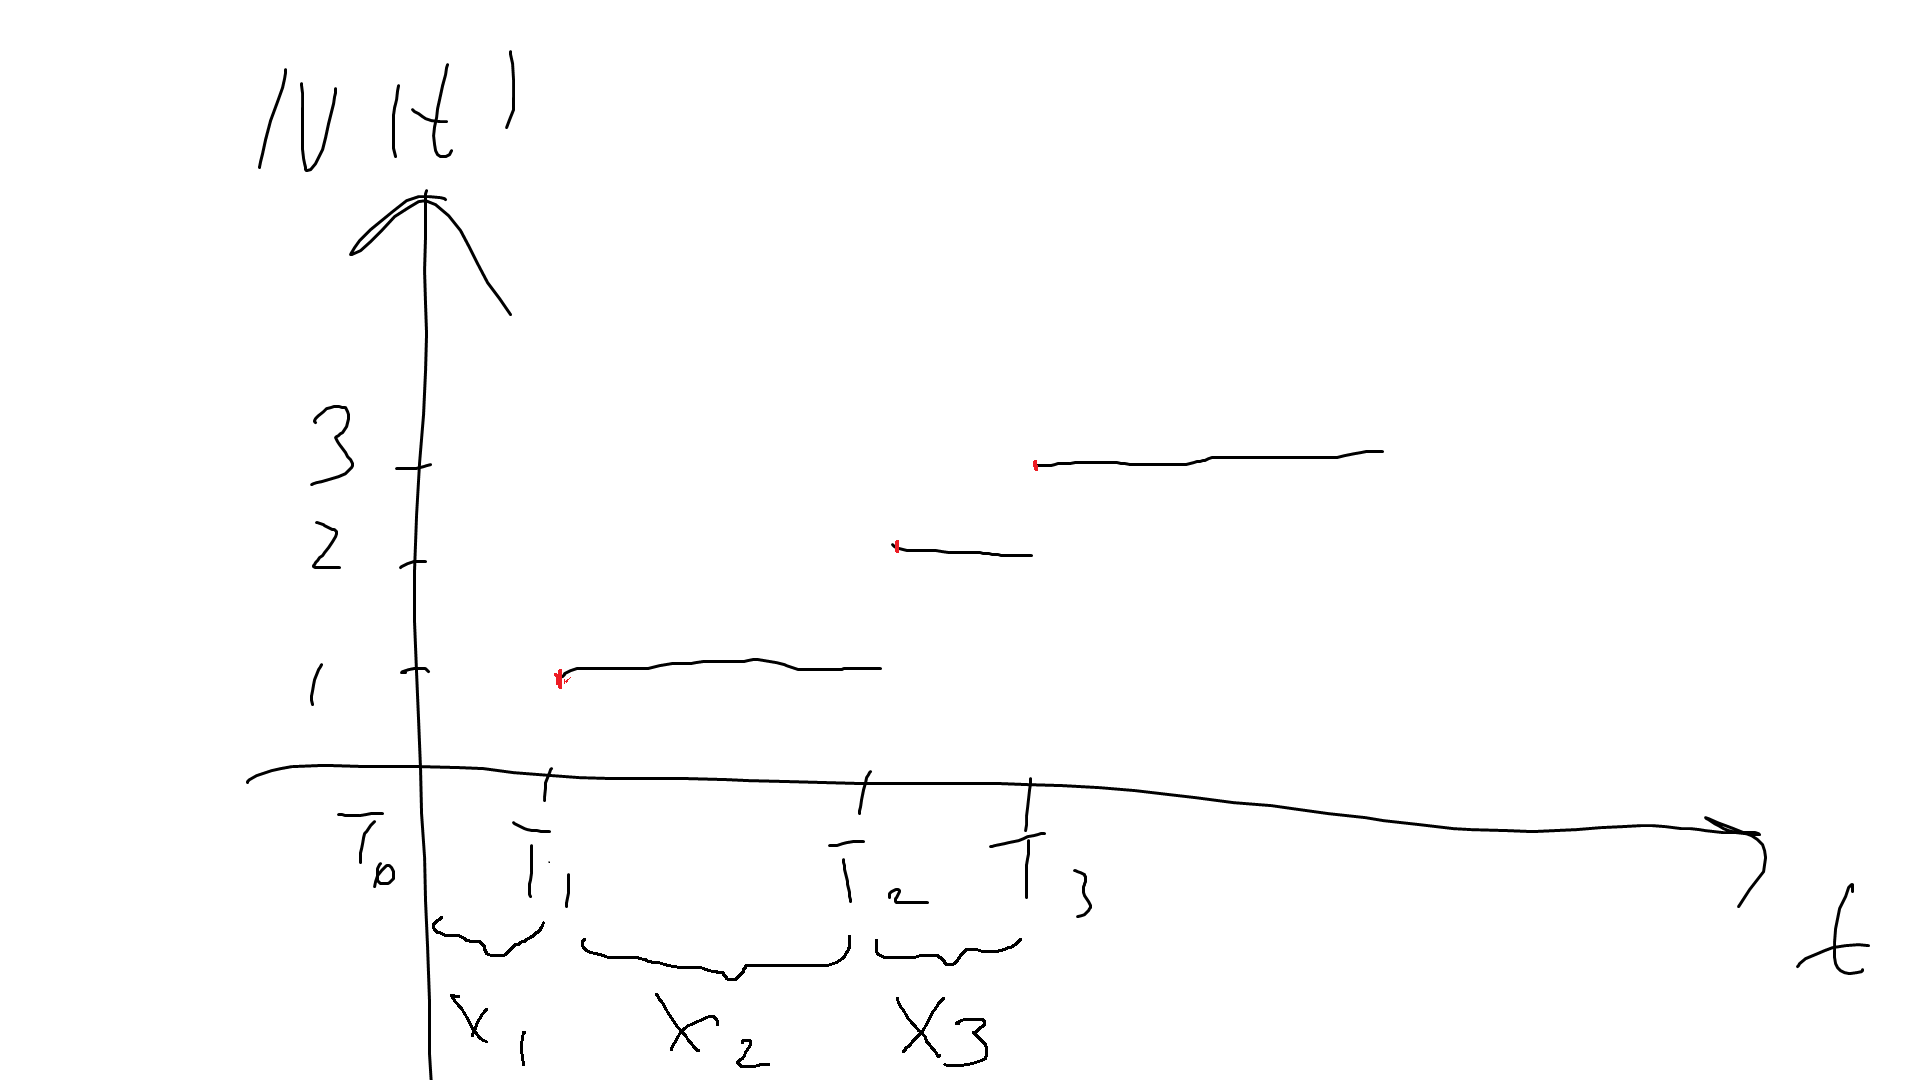
\includegraphics[scale=0.5]{image/AP_01.png}

\begin{thm}
Suppose $X_1,X_2,...$ are known. Let $T_n = \sum_1^n x_i$, note $N(t) = \max\{n:T_n \leq t\}$. Then the random variables $X_1,X_2,...$ are independent and they have the exponential distribution with parameter $\lambda$ ($Exp(\lambda)$).
\begin{proof}
\begin{equation*}
\begin{aligned}
\P(X_1 > t) = \P(N(t) = 0) = e^{-\lambda t}
\end{aligned}
\end{equation*}
So $X_1$ has $Exp(\lambda)$ distribution. Now consider $\P(X_2>t|X_1=t_1)$. This doesn't look to make much sense as $X_1$ has a continuous distribution so $\P(X_1=t_1) = 0$; however we could could consider the conditional densiy as $f_{X|Y} (x|y) =\frac{f_{X,Y}(x,y)}{f_Y(y)}$. Then $\P(X_2>t|X_1=t_1) = \P($ no arrivals in $(t_1,t_1+t)|X_1=t_1) = \P($ no arrivals in $(t_1,t_1+t)$ by independence. This is then equal to $\P($ no arrivals in $(0,t)) = \P(N(t)=0) = e^{-\lambda t}$. Then continue by induction.
\end{proof}
\end{thm}

\begin{prop} (properties of a poisson process $N$)\\
(a) $N$ has stationary independent increments, i.e.:\\
(i) If $0<t_1<...<t_n$, then $N(t_1),N(t_2)-N(t_1),...,N(t_n)-N(t_{n-1})$ are independent;\\
(ii) $N(s+t)-N(s) \xrightarrow{d} N(t)-N(0)$.\\
Amongst processes which are right continuous, non-decreasing, has only jump discontinuities of size 1, (i) and (ii) are characteristics of the Poisson process, meaning that Poisson process is the only process that has those two properties.\\
(b) Thinning:\\
Suppose insects arrive as a poisson process with parameter $\lambda$. Each insect is a mosquito with probability $\alpha$, or a skeet with probability $1-\alpha$, and the occurences of the two insects are independent. Then\\
(i) the mosquito-arrival process $F$ is a $PP(\alpha\lambda)$, 
(ii) the skeet-arrival process is $S$ a $PP((1-\alpha)\lambda)$, and 
(iii) these processes are independent.
\begin{proof}
(i) and (ii) are immediate by infinitestimal definition of a poisson process. For (iii), by independence we mean that $\P(F(t_1)=f_1,S(t_1)=s_1,...,F(t_n)=f_n,S(t_n)=s_n) = \P(F(t_1)=f_1,...,F(t_n)=f_n) \P(S(t_1)=s_1,...,S(t_n)=s_n)$ $\forall t_1,...,t_n,f_1,...,f_n,s_1,...,s_n)$.

The simple case is 
\begin{equation*}
\begin{aligned}
\P(F(t) = f, S(t) = s) &= \frac{(\lambda t)^{f+s} e^{-\lambda t}}{(f+s)!}{{f+s} \choose f} \alpha^f (1-\alpha)^s\\
&= \frac{(\alpha\lambda t)^f}{f!} e^{-\alpha\lambda t} \frac{((1-\alpha) \lambda t)^s}{s!} e^{-(1-\alpha)\lambda t}\\
&= \P(F(t) = f) \P(S(t) = s)
\end{aligned}
\end{equation*}
\end{proof}
(c) Superposition:\\
$F$: Flies arrive as $PP(\lambda_1)$;\\
$S$: Skeets arrive as $PP(\lambda_2)$, and these processes are independent. Then $N=F+S$ is a $PP(\lambda_1+\lambda_2)$. This follows by infinitesimal construction of $PP$.\\
(d) Given $N(t) = n$, write $\mathbf{T} = (T_1,...,T_n)$, $\mathbf{t} = (t_1,...,t_n)$, we have $f_{\mathbf{T}}(\mathbf{t} | N(t) = n) =\left(\frac{1}{t}\right)^n n! L(\mathbf{t})$, where $L(\mathbf{t})=1$ iff $t_1<t_2<...<t_n$.
\begin{proof}
Next time.
\end{proof}
\end{prop}

Let's complete the proof left last lecture.

\begin{thm}
Conditional on $\{N(t) = n\}$, the times $T_1,...,T_n$ have joint pdf
\begin{equation*}
\begin{aligned}
f_{ \mathbf{T} |N(t) = n} (\mathbf{t}) = \frac{n!}{t^n} L(\mathbf{t}) 1_{\{t_n \leq t\}}
\end{aligned}
\end{equation*}
where $L(\mathbf{t}) = 1_{\{t_1 \leq t_2 \leq ... \leq t_n\}}$.
\begin{proof}
The interarrival times $X_1,X_2,...,X_n$ have joint pdf
\begin{equation*}
\begin{aligned}
f_\mathbf{X}(\mathbf{x}) = \lambda^n \exp(-\lambda \sum_i^n x_i)
\end{aligned}
\end{equation*}
by change of variables, we now have (noting $T_i = X_1+...+X_i$)
\begin{equation*}
\begin{aligned}
f_\mathbf{T} (\mathbf{t}) = \lambda^n e^{-\lambda t_n} L(\mathbf{t})
\end{aligned}
\end{equation*}
Now for $C \subseteq \R^n$, we have
\begin{equation*}
\begin{aligned}
\P(T \in C | N(t) = n) &= \frac{\P(T \subseteq C, N(t) = n)}{\P(N(t) = n)}\\
&= \frac{1}{\P(N(t)=n)} \int_C \P(N(t)\\
&= n | \mathbf{T} = \mathbf{t} ) f_\mathbf{T} (\mathbf{t}) d \mathbf{t}\\
&= \frac{1}{\P(N(t) = n)} \int_{t_n \leq t} e^{-\lambda (t-t_n)}\lambda^n e^{-\lambda t_n} L(\mathbf{t}) d\mathbf{t}
\end{aligned}
\end{equation*}
the last equation is because we need ther to be no arrival between $t$ and $t_n$. Now the conditional pdf of $\mathbf{T}$ given $N(t) = n$ is
\begin{equation*}
\begin{aligned}
\frac{1}{(\lambda t)^n e^{-\lambda t} / n!} e^{-\lambda (t-t_n)} \lambda^n e^{-\lambda t_n} L(\mathbf{t}) = \frac{n! L(\mathbf{t})}{t^n} 1_{\{t_n \leq t\}}
\end{aligned}
\end{equation*}
I think somewhere in this proof we used $\P(X \in C) = \int_C g(u) du \iff f_X(u) = g(u)$, otherwise the lecture wouldn't have written this down on a separate board.
\end{proof}
\end{thm}

\newpage

\section{Continuous-time Markov chains}

This is actually quite a complicated topic, so we are going to make a lot of assumptions to simplify it.

Assume state space $S$ is countable, and we often take $S \subseteq \Z = \{ ...,-1,0,1,...\}$ (sometimes useful to assume $|S|<\infty$).

\begin{defi}
A process $X = \{X(t) : t \geq 0\}$ taking values in $S$ satisfies the \emph{Markov property} if:\\
\begin{equation*}
\begin{aligned}
\P(X(t_n) = j| X(t_1) &= i_1,...,X(t_{n-1}) = i_{n-1}) \\
&= \P(X(t_n) = j| X(t_{n-1}) = i_{n-1})
\end{aligned}
\end{equation*}
for all $i_1,i_2,...,i_{n-1}, j \in S, t_1< t_2 < ... < t_n$.

We have the transition probabilities $p_{i,j}(s,t) = \P(X(t) = j| X(s) = i)$. We, however, assume the process is homogeneous, i.e. $$p_{i,j}(s,t) = p_{i,j} (0,t-s) := p_{i,j}(t-s) \forall s,t,i,j$$so the transition probabilities only depend on the duration of time passed instead of the absolute time. We can then write this as a transition matrix $(p_{i,j}(t))_{i,j \in S}=P_t$.
\end{defi}

\begin{prop}
The family $\{P_t: t \geq 0\}$ satisfies\\
(a) $P_0 = I$;\\
(b) $P_t$ is a \emph{stochastic} matrix, i.e. a non-negative matrix with row sum 1;\\
(c) $P_{s+t} = P_s P_t$ for $s,t \geq 0$.
\begin{proof} (of (c))\\
$p_{i,j}(s+t) = \sum_{k \in S} p_{i,k}(s)p_{j,k}(t)$ by Markov Property which is just the component form of $P_{s+t} = P_s P_t$.\\
$P_{s+t} = P_s P_t$ is sometimes called the \emph{semigroup property} ($s,t \geq 0$).\\
$(P_t:t \geq 0)$ is called a \emph{stochastic semigroup}.
\end{proof}
\end{prop}

General theory involves conditions of regularity.

We assume $X$ is a right-continuous jump process.

Holding times for general chains:

Assume $X(t_0) = i$.\\
Let $H=\inf\{t>t_0:X(t) \neq i\}$. We have $$\P(H>u+v|H>u) = \P(H>v) \ (*)$$ by Markov Property ($u,v \geq 0$).\\
Let $G(u) = \P(H>u)$. By (*), we get $\frac{G(u+v)}{G(u)} = G(v)$, so $G(u+v) = G(u)G(v)$.\\
We know $G(0) = 1$, and $G$ is non-increasing.\\
Solution: $G(n) = G(1)G(n-1) = G(1)^n$ $\forall n \in \N$. Also $G(p/q)... G(p/q) =G(p) = G(1)^p$ so $G(p/q) = G(1)^{p/q}$, hence $G(u) = G(1)^u$ for $u \geq 0$. We deduce that $G(u) = e^{-\alpha u}$ for some $\alpha>0$.

\begin{lemma}
A random variable $X>0$ has an exponential distribution iff it has the \emph{lack of memory property}: $\P(X>u+v|X>u) = \P(X>v)$ $\forall u,v > 0$.
\end{lemma}

A MC s a combination of exponential-distribution holding times, and a transition matrix for the \emph{jump chain} $Y=(Y_n)$ given by $Y_0 =X(0)$, $Y_1 = X(T_1)$, where $T_1 = \inf\{t:X(t) \neq X(0)\}$, and $Y_n = X(T_n)$ where $T_{n+1} = \inf \{t > T_n: X(t) \neq X(T_n)\}$. $Y$ is a \emph{discrete-time Markov chain.}

If in state $i$, want $H$, we jump to state $j\neq i$ with probability $\frac{g_{ij}}{\alpha_i}$. Intensity of a jump is $\alpha_i$, and intensity of a jump to state $j$ is $g_{ij}$.\\
Note a transition from $i$ to itself is not deemed to be a transition.

We have $p_{ij} (h) = g_{ij} h + o(j)$ ($j \neq i$), $p_{ij}(h) = 1- \sum_{j \neq i} p_{ij}(h) = 1-h\sum_{j \neq i} g_{ij} + o(h) = 1-\alpha_i h + o(h) = 1+g_{ii} h + o(h)$, where we let $g_{ii} = -\alpha_i$. Now we let $G$ be the matrix $(g_{ij})$, with the off-diagonal terms the previous $g_{ij}$'s, but the diagonal terms $g_{ii}$ as defined just now (so as to make row sums 0). Now the off-diagonal terms are non-negative, and diagonal terms are non-positive. We call $G$ the \emph{generator} of the chain (otherwise known as the $Q$-matrix).

Conclusion: $\frac{P_t - I}{t} \xrightarrow{t \to 0^+} G$.\\
Questions of regularity: OK if $|S| < \infty$.

(?)
\begin{equation*}
\begin{aligned}
p_{ij}(t+h) &= \sum_k p_{ik}(t) p_{kj}(h)\\
&= \sum_{k \neq j} p_{ik}(t) [g_{kj} h + o(h) + p_{ij}(t) (1+g_{jj} h + o(h))\\
&= \sum_k p_{ik} (t) g_{kj}\\
&= P_t \cdot G
\end{aligned}
\end{equation*}
this is the (Kolmogov) Forward Equation.

$p_{ij}(t+h) = \sum_k p_{ik}(h) p_{kj}(t)$, so $P't = GP_t$, called the K-Backward equation.

Interchange of limits requires justification -- it's OK if $|S| < \infty$.

Now $P'_t = P_t G$, we can rewrite this as $f'=fg$, which gives $f(t) = A e^{gt}$. So the solution should be $P_t = P_0(=I)e^{tG}$ (i.e. $=\sum_{k=0}^\infty \frac{t^k}{k!} G^k$).

In many cases, the solution to the forward and/or backward equation is the function $P=e^{tG}$.

A mistake has been made! The definition for holding time is wrong. It should be $H=\inf\{ t-t_0: X(t) \neq X(t_0), t > t_0\}$ (the length rather than the absolute time).

Let's look at an example now.
\begin{eg}
Let $S=\{1,2\}$, $G={{-\alpha \ \alpha} \choose {\beta \ -\beta}}$, where $\alpha\beta > 0$. What are the $p_{ij}(t)$?\\
There are only two states, so let's find
\begin{equation*}
\begin{aligned}
p_{11}'(t) = -\alpha p_{11} + \beta p_{12},\\
p_{12}'(t) = \alpha p_{11}(t) - \beta p_{12}(t)\\
...
\end{aligned}
\end{equation*}
So we get a bunch of differential equations, with boundary conditions $p_{11}(0) = p_{22}(0) =1$. This has a unique solution (check). We get $P_t = e^{tG} =\sum_n \frac{t^n}{n!} A \Lambda^n A^{-1}$ wher we diagonalize $G=A\Lambda A^{-1}$. But $e^{t\Lambda}$ is equal to $Diag(e^{\lambda_1 t}, e^{\lambda_2 t} ...)$. Each $p_{ij}(t)$ has the form $\sum_k e^{\lambda_k t} c_K (i,j)$, where we need to find the constants $c_k(i,j)$.
\end{eg}

\begin{lemma}
Let $i,s \in S$. Then either $p_{ij}(t)=0$ $\forall t>0$, or $p_{ij}(t) > 0$ $\forall t > 0$ (this is because our time here is continuous; we can fit in any number of jumps in any time length with positive probability).
\begin{proof}
Assume $p_{ij}(T) > 0$ for some $T>0$. Then for $t>T$, $p_{ij}(t) \geq p_{ij}(T) \P_j (X_j > t-T) > 0$ (start in $j$ and holding time $> t-T$, which is positive).\\
For $t<T$: there exists finite sequence of jumps from $i$ to $j$ in time $T$, so there exists $i_1,i_2,...,i_n \in S$ with $g_{i,i_1}g_{i_1,i_2}...g_{i_n,j}>0$, where $g_{i,j}$ is as defined previously. Then we can just divide the time $(0,t)$ into $n+1$ intervals. Then $p_{i,j}(t) \geq p_{i,i_1}(t/(n+1))...p_{t_n,j}(t/(n+1)) > 0$ (this is an applied course, so we don't care that much).
\end{proof}
\end{lemma}

\begin{defi}
The chain $X$ on state space is \emph{irreducible} if $\forall i,j \in S$, $\forall t > 0, p_{i,j}(t)>0$ ($\iff \exists t>0, p_{i,j}(t)>0$).
\end{defi}

A distribution $\pi$ on $S$ is invariant (or stationary, or equilibrium distribution) if $\pi = \pi P_t$ for all $t \geq 0$.

Note: if $X(0)$ has distribution $\mu_0$, then $X(t)$ has distribution $\mu_t = \mu_0 P_t$ ($\mu_t(j) = \sum_i \mu_0(i) p_{i,j}(t)$).

Note: (a) Differentiate $\pi = \pi P_t$ to get $0 = \pi G$;\\
(b) If $P_t = e^{tG}$ then $\pi G = 0$ iff $\pi G^n = 0$ for $n \geq 1$ iff $\pi \sum_n \frac{t^n}{n!} G^n = \pi$ iff $\pi P_t = \pi$.

\begin{thm}
Let $X$ be irreducible. If there exist an invariant distribution $\pi$, then it is unique (what a surpise), and $p_{ij}(t) \to \pi_j$ as $t\to \infty$. Can we prove this in the remaining 11 minutes? Let's try:
\begin{proof}
Let $h>0$. Then $Y_n=X(nh)$. So $Y$ is a 'skeleton' of $X$. $Y$ is a markov chain. Since $X$ is irreducible, so is $Y$. $Y$ has invariant distribution $\pi$, hence $\pi$ is unique. (?) Since $X$ is irreducible, $Y$ is aperiodic(?). Hence $p_{ij}(nh) \to \pi_{ij}$ as $n \to \infty$. Since this holds for all $h \in \Q^+$, we deduce that $p_{ij}(t) \to \pi_j$ as $t\to \infty$ through the rationals. The conclusion follows by continuity of $p_{ij}(\cdot)$.
\end{proof}
\end{thm}

\begin{lemma}
The functions $p_{ij}(\cdot)$ are continuous.
\end{lemma}

Last time we claimed that if $\forall h>0$, $p_{ij}(nh) \pi_j$ as $n \to \infty$, then $p_{ij}(t) \to \pi_j$ as $t \to \infty$. However this is wrong as the rate of convergence might depend on $h$.\\
From some theorem in Linear Analysis it is known that if $p$ is continuous then the above is actually true. But this is an applied course so let's not assume Linear Analysis. Let's now prove it with the following lemma:
\begin{lemma}
$p_{ij}(\cdot)$ is uniformly continuous in $t$.
\begin{proof}
\begin{equation*}
\begin{aligned}
|p_{ij}(t+h)-p_{ij}(t)| &= |[\sum_k p_{ik}(h) p_{kj}(t)] - p_{ij}(t)|\\
&\leq |\sum_{k \neq i} p_{ik}(h) p_{kj}(t) | + |p_{ij}(t) [1- p_{ii}(h)]|\\
&\leq [1-p_{ii}(h)]\\
&\leq 2(1-e^{-g_i h}) \to 0
\end{aligned}
\end{equation*}
as $h \to 0$.
\end{proof}
\end{lemma}
Back to the theorem: let $t>0$, $\exists h$ s.t. $|p_{ij}(t+h) - p_{ij}(t)| < \frac{1}{2}\varepsilon \forall t$. Then $|p_{ij}(t) - p_{ij}(\lfloor t/h \rfloor h)| < \frac{1}{2} \varepsilon$. Pick $N$ s.t. $|p_{ij}(nh) -\pi_j| < \varepsilon/2$ for $n \geq N$. For $t>(n+1)h$ we have $|p_{ij}(t) - \pi_j| \leq |p_{ij}(t) - p_{ij}(\lfloor t/h\rfloor h)| + |p_{ij}(\lfloor t/h \rfloor h) - \pi_j) \leq \frac{1}{2}\varepsilon + \frac{1}{2} \varepsilon$ so done.

\emph{Explosion}:\\
Let $S$ be countable. $H=(h_{i,j}:i,j \in S)$ is the transition matrix of a discrete time markov chain $Z = (Z_n : n \geq 0)$ on $S$. Assume $h_{i,i} = 0 \forall i \in S$. Let $(g_i:i \in S)$ be non-negative reals. Inifinitesimal definition of $X$: $g_{ij} = g_i h_{ij}$ if $i \neq j$, and $-g_i$ if $i=j$. Holding time definition: $X(0) = Z_0$. Given $Z$, let $U_0,U_1,...$ be independent exponential random variables, where $U_n$ has parameter $g_{Z_n}$.

We define $T_n = U_0 + ... + U_{n-1}$, the time of the $n^{th}$ jump. $X(t) = Z_n$ if $T_n \leq t < T_{n+1}$.

$T_n \to T_\infty = \sum_0^\infty U_n$. Say the process [explodes if $T_\infty < \infty]$, or explodes if $\P(T_\infty < \infty) > 0$.

We augment the state space $S$ to $S' = S \cup \{\infty\}$ (cemetery state, means $\infty$ is absorbing). Assume: at $T_\infty$, the chain enters the cemetery state labelled $\infty$. Such a process is called minimal.

\begin{thm}
The process $X$, constructed via holding times as above, does not explode if any of the following occurs:\\
(a) $|S| < \infty$;\\
(b) $\sup_i g_i < \infty$;\\
(c) $X(0) = i$, where $i$ is recurrent for the jump chain $Z$.
\end{thm}

\begin{lemma}
Let $X_1,...$ be independent random variales, and $X_i$ has distribution $Exp(\lambda_{i-1})$. Let $T_\infty = \sum_1^\infty X_i$. $\P(T_\infty < \infty = 0$ if $\sum \lambda_i^{-1} = \infty$, and 1 otherwise.
\begin{proof}
\begin{equation*}
\begin{aligned}
\E(T_\infty) &= \E(\sum_1^\infty X_i)\\
&= \E (\lim_{N \to \infty} \sum_1^N X_i)\\
&= \lim_{N \to \infty} \E(\sum_1^N X_i)\\
&= \lim_{N \to \infty} \sum_1^N \frac{1}{\lambda_{i-1}}\\
&= \sum_1^\infty \frac{1}{\lambda_{i-1}}
\end{aligned}
\end{equation*}
Now If $\sum \frac{1}{\lambda_{i-1}} < \infty$, then $\E(T_\infty) < \infty$. So $\P(T_\infty = \infty) = 0$.\\
The other part will be proven in next lecture.\\
Problem sheet 2 is online!\\
For the other part we have 
\begin{equation*}
\begin{aligned}
\E(e^{-T_\infty}) &= \E(\prod_1^\infty e^{-X_i})\\
&= \prod_1^\infty \E(e^{-X_i})\\
&= \prod_1^\infty \frac{1}{1+\lambda_i^{-1}} = 0
\end{aligned}
\end{equation*}
the second equation by dominated convergence. So $\P(e^{-T_\infty} = 0) = 1$.
\end{proof}
\end{lemma}

Proof of theorem:
\begin{proof}
(a) to (b):(proved? where) \\
Proof that (b) implies no explosion:\\
Suppose $g+i \leq \gamma < \infty$ for some $\gamma$. Then $\sum_0^\infty$ is a sum of independent exponential distribution r.v.s, i.e .$U_i \sim Exp(g_{z_i})$. hence $g_{Z_i} U_i \sim Exp(1)$.\\
Now $\gamma \sum_0^\infty U_i \geq \sum_i g_{Z_i} U_i$ is sum of independent $Exp(1)$ random variables, which diverges with probability 1. So $\P(T_\infty < \infty) = 0$.\\
Proof that (c) implies no explosion: We know there are infinitely many $n$ with $Z_n = i$ (a.s.) since $i$ is recurrent. Now $T_\infty \geq$ sum of infinitely many indepnedent holding times in state $i$ = sum of independent $Exp(g_i)$ random variables which diverges a.s.. So $\P(T_\infty < \infty) = 0$.
\end{proof}

\begin{eg}
Let $Z$ be a discrete-time chain with transition matrix $H$, where $H_{i,i} = 0$ $\forall i \in S$. Let $N$ be a PP with intensity $\lambda>0$.\\
Let $X(t) = Z_n$ if $T_n \leq t < T_{n+1}$, where $T_n$ is the time of the $n^{th}$ arrival in $N$. Now
\begin{equation*}
\begin{aligned}
p_{ij}(t) &= \sum_{n=0}^\infty \P(X(t) = j | X(0)=i,N(t) = n) \P(N(t) = n)\\
&= \sum_n \frac{(\lambda t)^n}{e^{-\lambda t}}{n!} (H^n)_{i,j}
\end{aligned}
\end{equation*}
We have
\begin{equation*}
\begin{aligned}
e^{\lambda t} I = \sum_{n=0}^\infty \frac{(-\lambda t)^n}{n!} I^n = e^{-\lambda t I}
\end{aligned}
\end{equation*}
So $P_t = e^{\lambda t(H-I)^n} = e^{tG}$ where $G=\lambda(H-I)$.
\end{eg}

\begin{defi}
State $i$ of the continuous time MC $X$ is recurrent if $\P_i(\{t \geq 0: X(t) = i\}$ is unbounded$)=1$; it is transient if the above probability is 0.
\end{defi}

\begin{thm}
(a) If $g_i = 0$, then $i$ is recurrent.\\
(b) Let $g_i>0$. State $i$ is recurrent for $X$ if it is recurrent for the jump chain $Z$. Furthermore, $i$ is recurrent if 
\begin{equation*}
\begin{aligned}
\int_0^\infty p_{ii}(t) dt = \infty
\end{aligned}
\end{equation*}
\begin{proof}
(a) If $g_i = 0$ then $\{(X(t) = i, \forall t) = 1$.\\
(b) Let $g_i>0$. If $i$ is transient for $Z$, then $Z$ has a last visit to $i$ at some time $N$. So $X(t) \neq i$ for $t>T_{N+1}$. So $i$ is transient for $X$. If $i$ is recurrent for $Z$, the times at which $Z$ visits $i$ is infinite a.s.. By last theorem, there is no explosion. So the chain $\{T_n:Z_n=i\}$ is unbounded a.s.. ($T_n$ is time of $n^{th}$ jump of $X$). Hence $i$ is recurrent for $X$.
Note: the proof implies a non-recurrent state is transient.\\
Now
\begin{equation*}
\begin{aligned}
\int_0^\infty p_{ii}(t) dt &= \int_0^\infty \E_i(1_{X(t) = i}) dt\\ 
&= \E_i (\int 1_{X(t)=i} dt) \\
&= \E_i(\sum_n U_n 1_{\{Z_n=i\}})\\
&= \sum_n \frac{1}{g_i} \P_i (Z_n = i)\\
&= \frac{1}{g_i} \sum_n (H^n)_{i,i} = \infty
\end{aligned}
\end{equation*}
if $i$ is recurrent for $Z$.
\end{proof}
\end{thm}

Assume $g_j>0 \forall j$. $g_i=0$.

\newpage
\section{Birth Process}
This is a continuous-time Markov Chain with generator $g_{n,n+1} = \lambda_n$ and $g_{n,m} = 0$ for $m \neq n,n+1$. When in state $n$, we jump to $n+1$ at rate $\lambda_n$, otherwise stay at $n$. $\lambda_n$ is just a constant, so if $\lambda_n=\lambda$ $\forall_n$ then this is just a Poisson process.

For a \emph{simple birth process}, living particles give birth to single offspring at rate $\lambda$ independently of other offsprings.\\
Let $N_t =$ number of individuals alive at time $t$. Then
\begin{equation*}
\begin{aligned}
\P(N_{t+h} = n+m | N_t = n) = {n \choose m} (\lambda h+o(h))^m (1-\lambda h -o(h) )^{n-m} + o(h) = \left\{\begin{array}{ll}
1-n\lambda h + o(h) & m=0\\
n\lambda h + o(h) & m=1\\
o(h) & m \geq 2
\end{array}
\right.
\end{aligned}
\end{equation*}
Hence this is a birth process with $\lambda_n = n\lambda$.

Let's look at another example:

\begin{eg}
Simple birth with immigration: in this model we have $\lambda_n = n\lambda + \varepsilon$, where $\lambda$ is the birth rate and $\varepsilon$ is the immigration rate.

Kolmogorov equations:\\
Forward equation: condition on $N_t$, $p'_{ij}(t) = \lambda_{j-1} p_{i,j-1}(t) - \lambda_j p_{ij}(t), i,j \geq 0, t \geq 0$, so $P'_t = P_t G$.\\
Backward eqautions: condition on $N_h$, $p'_{ij}(t) = \lambda_i p_{i+1,j}(t) - \lambda_i p_{i,j}(t)$. So $P'_t = GP_t$.\\
Boundary condition: $p_{i,j}(0) = \delta_{i,j}$.\\
Facts: $p_{i,i-1}(t) = 0$.
\end{eg}

\begin{thm}
For a birth process, the forward equations have a unique solution, which satisfies the backward equation.
\begin{proof}
$j=i$ in Forward equation: $p_{ii}'(t) = -\lambda_i p_{i,i}(t)$. Hence $p_{ii}(t) = e^{-\lambda_i t}$,\\
$p_{i,i+1}'(t) = \lambda_i p_{i,i}(t) - \lambda_{i+1} p_{i,i+1}(t)$.\\
Hence $p_{i,i+1}(t)$ and hence $p_{i,j}(t)$ by induciton.
\end{proof}
\end{thm}

Laplace transforms:\\
Let $g:\R^+ \to \R$. We define the laplace transform of $g$,
\begin{equation*}
\begin{aligned}
\hat{g}(\theta) = \int_0^\infty e^{-\theta t} g(t) dt
\end{aligned}
\end{equation*}
for $\theta > 0$.

Remember we have the mgf, $E(e^{\theta x}) = \int e^{\theta t} f_x(t) dt$.

We have the Laplace inverse theorem (in Complex Methods). We know
\begin{equation*}
\begin{aligned}
\int e^{-\theta t} g'(t) dt = [e^{-\theta t} g]_0^\infty + \int \theta e^{-\theta t} g(t) dt\\
&= -g(0) + \theta \hat{g}(\theta) = \hat{g'}
\end{aligned}
\end{equation*}

Now
\begin{equation*}
\begin{aligned}
&\theta \hat{p}_{ij} - \delta_{i,j} = \lambda_{j-1} \hat{p}_{i,j-1} - \lambda_j \hat{p}_{i,j}\\
&\implies (\theta+\lambda_j) \hat{p}_{ij} = \delta_{i,j} + \lambda_{j-1} \hat{p}_{i,j-1}
\end{aligned}
\end{equation*}
hence the $\hat{p}_{i,j}$'s are
\begin{equation*}
\begin{aligned}
\hat{p}_{ij}(\theta) = \frac{1}{\lambda_j} \frac{\lambda_j}{\theta+\lambda_i} ... \frac{\lambda_j}{\theta+\lambda_j}, i \leq j.
\end{aligned}
\end{equation*}

It's easy to check that this Laplace transform satisfies the "Laplace" equation of the backward "system",
\begin{equation*}
\begin{aligned}
-\delta_{ij} + \theta \hat{p}_{ij} = \lambda \hat{p}_{i+1,j} -\lambda_j \hat{p}_{i,j}
\end{aligned}
\end{equation*}

\begin{thm}
The forward equations have a unique solution $(p_{i,j}(t))$ which is the minimal solution to the backward equation, in that, for any other solutions $(\pi_{i,j}(t))$ to the backward equation, we have
\begin{equation*}
\begin{aligned}
p_{i,j}(t) \leq \pi_{i,j}(t) \forall i,j,t
\end{aligned}
\end{equation*}
The lecture thinks the proof might be in a book of Norris, or online notes by Burostychi + Sousi(?).
\end{thm}

If we know in addition that $\sum_j p_{i,j}(t) = 1$ $\forall i$, then we know $p_{i,j}(t)$ is the unique solution to the backward equation, as any other solution $\pi_{i,j}(t)$ would have a sum exceeding 1.

Assume we have a MC $X=(X(t))$, and jump chain $Y=(Y_n)$. Assume $g_j>0$ $\forall j$. Speaking (probably not this word) $X$ via holding time definition. Assume $X$ is a minimal process. We can define the transition probability: 
\begin{equation*}
\begin{aligned}
p_{i,j}(t) = \P_i(X(t)=j) \forall i,j \in S
\end{aligned}
\end{equation*}
The $(p_{i,j}(t))$ satify the C-K equations.

Something we've talked about in the last lecture:

(a) $(p_{i,j}(t))=P_t$ is the minimal no-negative solution to forward equation $P_t' = P_tG$, $P_0 = I$. Here minimal: for any non-negative solution $\pi$ we have $p_{i,j}(t) \leq \pi_{i,j}(t)$ $\forall i,j,t$;\\
a
(b) $P_r$ is the minimal non-negative solution to the backward equation $P'_t=GP_t$, $P_0=I$.

\subsection{Strong Markov Property}
A \emph{Stopping time} is a random variable $T$ taking values in $[0,\infty) \cup \{\infty\}$ such that $\{T \leq t\} \in \mathcal{F}_T = \sigma(\{X(s):s\leq t\})$, the smallest $\sigma$-algebra on which every $X(s)$ for $s\leq t$ is measurable.

Strong Markov Property: Let $X$ be a MC, with given generator and initial distribution. Let $T$ be a stopping time for $X$. Given $T<S$, and $X(T) = i$. Then $\{X(T+t):t \geq 0\}$ is a MP with generator $G$ and initial state $X(T) =i$, which is independent of $\{X(s):s \leq T\}$.\\
The proof is omitted for measure-theoretic reasons.

Hitting times: Let $X$ be a MC, as usual, with generator $G$. Hitting time of $A \subseteq S$ is $T_A = \inf \{t \geq 0: X(t) \in A\}$.

Note: $T_A$ is a stopping time. The jump chain $Y$ has hitting time $H_A= \inf\{n \geq 0:Y_n \in A\}$. Now $\{T_A < \infty\} = \{H_A < \infty\}$. We call $h_A(i) = \P_i(T_A < \infty)$ (starting in $i$). Then $h_A(i) = \P_i(H_A < \infty)$. Hence $h_A$ is least non-negative solution to $h_A(i) = 1$ if $i \in A$, $h_A (i) = \sum_{j \in S} \frac{g_{i,j}}{g_i} h_A(j)$ if $i \not\in A$\\
i.e. $h_A$ satisfies the equations, and $h+A(i) \leq h'_A(i)$ $\forall i$ for any other non-zero solution $h'_A$.

$-g_{i,i}h_A(i) = \sum_{j \neq i} g_{i,j} h_A(j)$, i.e. $Gh_A = 0$.

Hence $h_A$ is the least non-negative solution to:\\
$h_A(i) = 1$ if $i \in A$,\\
$Gh_A(i) = 0$ if $i \not\in A$.

Let $k_A(i) = \E_i(T_A)$, and assume $h_A(i) = 1$ $\forall i$. $k_A(i) = 0$ if $i \in A$. Let $i \not\in A$. Then $k_A(i) = \frac{1}{g_i} + \sum_{j \neq i} \frac{g_{i,j}}{g_i} k_A(j)$. By SMP, $-g_{ii}k_A(i) = 1+\sum_{j \neq i} g_{ij} k_A(j)$, so $Gk_A(i) = -1$ for $i \not\in A$.

\begin{thm}
$k_A$ is minimal non-negative solution to $k_A(i) = 0$ if $i\in A$ and $Gk_A(i) = -1$ if $i \not\in A$.
\end{thm}

Invariant distributions:\\
Suppose we have a MC $X$, $\pi=(\pi_i:i \in S)$ is an invariant distribution if $\pi_i \geq 0$, $\sum_i \pi_i = 1$, and is invariant if $\pi P_t = \pi \forall t$.

\begin{thm}
Let $X$ be irreducible and recurrent. The distribution $\pi$ on $S$ satisfies $(\pi P_t = \pi \forall t)$ iff $\pi G=0$.
\begin{proof} (skeleton proof)\\
If $\pi P_t = \pi \forall t$, then $\pi P'_t = 0$ $\forall t$. When $t=0,\pi G = 0$. If $\pi G = 0$, by K-Backward equation, $\pi P'_t = (\pi G) P_t = 0$, so $\pi P_t =\ pi P_0 = \pi I = \pi$.
\end{proof}
\end{thm}

Positive recurrence: assume $g_j>0$ $\forall j$.

Let $U_i = \inf \{t>X-1:X(t) = i\}$. $i$ is recurrent if $\P_i (U_i < \infty) =1$. Easy to see this is equivalent to saying $\P_i(\{t:X(t) = i\}$ is unbounded $) = 1$. $i$ is positive (or non-null) recurrent if $\E_i(U_i) < \infty$.

\begin{thm}
Let $X$ be irreducible, with generator $G$. The following are equivalent:\\
(a) every state is positive recurrent;\\
(b) some state is positive recurrent;\\
(c) $X$ is non-explosive with invariant distribution $\pi_i = 1/g_im_i$ ($i \in S$).
\begin{proof}
(a) $\implies$ (b) is trivial.\\
Assume (b). Let $i$ be positive recurrent. Recurrence or not are shared properties of $X$ and $Y$ and irreducibility (??). So $i$ is recurrent for $X$ $\implies$ $i$ is recurrent for $Y$ (???), $X$ is irreducible implies $Y$ is. So every state is recurrent for $Y$, and so is for $X$.\\
In particular, $X$ starts in a recurrent state, so $X$ is non-explosive. Let $i$ be recurrent. Let $\mu_j = \E_i (\int_0^{U_i} 1(X_s = j) ds) = \frac{1}{g_j} \E_i ($number of visits by $Y$ to $j$ before 1st return to $i) = \frac{1}{g_j} v_i(j)$.

$v_i = (v_i(j) : j \in S)$ is invariant for $Y$ (this is not a distribution). Now
\begin{equation*}
\begin{aligned}
\sum_j \mu_j g_{jk} &= \sum_j \frac{v(j)}{g_j} [(h_{jk}-\delta_{jk})g_j] \\
&= v(k) - v(k) = 0
\end{aligned}
\end{equation*}
where $(h_{jk}$ is the transition matrix of $Y$. So $\mu G = 0$. 

$\sum_j \mu-j = m_i$.  Assuming that $i$ is positive recurrent, $m_i < \infty$, and hence $(\mu_j/m_i:j \in S)$ is an invariant distribution $\pi$. In particular, $\pi_i = 1/g_i m_i$.

Also, see the printed notes for proof.
\end{proof}
\end{thm}

\subsection{Reversibility}
Fact: If $X$ is a MC with generator $G$, $X$ irreducible $\iff$ $\forall i,j \in S, \exists i_1,i_2,...,i_n \in S$ distinct, with $g_{i,i_1}g_{i_1,i_2}...g_{i_n,j} > 0$ (also $i \neq i+1, i_n \neq j$).

--Lecture on 20180212: half an hour spent on the proof of positive recurrence and invariant distribution. See printed notes.

For an example, let's consider a birth-death process again, with $g_{n,n+1} = \lambda g_n$, $g_{n,n-1} = \mu g_n$, where we disallow jumping left from $0$, and $\lambda + \mu = 1$, $g_n > 0 \forall n$.

The jump chain is a simple random walk, i.e. jumps take values $\pm 1$. We know this SRW is recurrent if $\lambda \leq \mu$, and is positive recurrent if $\lambda < \mu$. Invariant measure for jump chain is $\rho_i = (\lambda/\mu)^i (1-\frac{\lambda}{\mu}$. Hence $X$ has invariant distribution $A(\lambda/\mu)^i/g_i$ for some constant $A$ by previous result (see printed notes).

When is this a distribution? Let's try some examples. If $g_i = g$ $\forall i$, then $X$ has an invariant distributon iff $\lambda < \mu$. Try another one: if $g_i = 2^i$, i.e. when we go further to the right, we move faster and faster, and suppose we have $1<\lambda/\mu<2$, then $X$ has an invariant distribution, since $\sum (\lambda/\mu)^i 1/2^i < \infty$.\\
In this case, $X$ has an invariant distribution, but the jump chain is not recurrent ($\lambda/\mu>1$) (the chain $X$ is exploding -- check).

\begin{thm}
Let $X=(X(t):t \geq 0)$ be an irreducible, non-explosive MC, with generator $G$ and invariant distribution $\pi$. In particular, $\pi G = 0$. Assume $X(0)$ has distribution $\pi$. Fix $T>0$, and let $\tilde{X}(t) = X(T-t)$. Then $\tilde{X}$ is a MC with initial distribution $\pi$, generator $\tilde{G} = (\tilde{g}_{ij})$ given by (detailed balance equation) $\pi_i g_{i,j} = \pi_j \tilde{g}_{ji}$ for $i,j \in S$.\\
$\tilde{X}$ is irreducible, non-explosive, with invariant distribution $\pi$.
\begin{proof}
$\tilde{G}$ is a generator since $\tilde{g}_{ij} \geq 0$ for all $i \neq j$ by (the detailed balance equation). Furthermore, $\sum_j \tilde{g}_{i,j} = \sum_j \pi_j \frac{g_{ji}}{\pi_i} = \frac{1}{\pi_i} 0 = 0$.\\
We'll complete the proof next time.\\
Now $\tilde{G}$ is a generator, we have
\begin{equation*}
\begin{aligned}
\tilde{p}_{ij} (t) &= \P (\tilde{X}(u+t) = j | \tilde{X}(u) = i)\\
&= \frac{\pi_j}{\pi_i} p_{ji}(t)
\end{aligned}
\end{equation*}
Now prove that $\tilde{X}$ is a MC:
\begin{equation*}
\begin{aligned}
P(\tilde{X}_{t_0} = i_0,\tilde{X}_{t_1} = i_1,...,\tilde{X}_{t_n} = i_n) &= \P(X(0) = i_n,X_{s_n} = i_{n-1},...,X_{s_1+...+s_n} = i_0)\\
&= \pi_{i_n} p_{i_n,i_{n-1}} (s_n)...p_{i_1,i_0} (s_1)\\
&= \pi_{i_0} \tilde{p}_{i_0,i_1} (s_1) ... \tilde{p}_{i_{n-1},i_n} (s_n)
\end{aligned}
\end{equation*}
for $t_0<t_1<...<t_n = T$, $i_0,...,i_n \in S$, $s_i = t_i - t_{i-1}$. Well hopefully this is correct. So $\tilde{X}$ is a MC with invariant distribution $\pi$.
\end{proof}
\end{thm}

$\sum_j p_{ij}(t) = 1$? $(p_{ij}(t))$ satisfies the forward equation $P'_t = P_t G$. Deduce $(\tilde{p}_{i,j}(t))$ satisfy backward equation $\tilde{P}'_t = \tilde{G}\tilde{P}_t$.\\
Proof that $\tilde{P}'_t = \tilde{G} \tilde{P}_t$:
\begin{equation*}
\begin{aligned}
p'_{ij}(t) &= \frac{\pi_j}{\pi_i} p'_{ji}(t) = \frac{\pi_j}{\pi_i} \sum_k p_{jk}(t) g_{ki}\\
&= \frac{\pi_j}{\pi_i} \sum_k \frac{\pi_k}{\pi_j}\tilde{p}_{kj}(t) g_{ki}\\
&= \sum_k \tilde{g}_{ik} \tilde{p}_{kj} (t)
\end{aligned}
\end{equation*}
So $\tilde{P}'_t = G\tilde{P}_t$.\\
We know $\sum_j \tilde{p}_{ij}(t) = \sum_j \frac{\pi_j}{\pi_i} p_{ji}(t) = \frac{1}{\pi_i}\pi_i = 1$. So $\tilde{X}$ is non-explosive, and $\tilde{P}'_t = \tilde{G}\tilde{P}_t$. So $\tilde{X}$ is a non-explosive MC with generator $\tilde{G}$. $\tilde{G}$ is irreducible since $G$ is.

\begin{defi}
$X$ is called reversible if, $\forall T>0$, the reversed process $\tilde{X}$ has the same distribution/law as $X$. Above, $X$ is reversible iff $\pi_i \tilde{g}_{ij} = \pi_j g_{ji}$, $i,j \in S$. This is called the \emph{detailed balance equation}.

We say $G,\lambda$ (generator and distribution) are in detailed balnce if the detailed balance equations hold.
\end{defi}

\begin{thm}
If $G,\pi$ are in detailed balance, then $\pi$ is invariant.\\
Note that the reverse is not necessarily true.
\begin{proof}
Check $\pi G = 0$:
\begin{equation*}
\begin{aligned}
\sum_i \pi_i g_{ij} = \sum_i \pi_j g_{ji} = \pi_j \times 0 = 0
\end{aligned}
\end{equation*}
\end{proof}
Note: in this case, if $X(0)$ has distribution $\pi$, then $X$ is reversible.
\end{thm}

\begin{eg} (Birth-death chains)\\
We have $g_{i,i+1} = \lambda_i$, $g_{i,i-1} = \mu_i$, $g_{ij} = 0$ if $|i-j| \geq 2$, and $g_{0,-1} =0$. Assume $\lambda_i,\mu_i > 0$ otherwise.\\
\end{eg}

Detailed balance equations:\\
$\pi_i g_{i,i+1} = \pi_{i+1} g_{i+1,i}$, $x_i \pi_i = \mu_{i+1} \pi_{i+1}$ with $i \geq 0$. Solve to obtain each $\pi_n$ in terms of $\pi_0$. $\pi$ is a distribution iff we can choose $\pi_0 \in (0,1)$ such that $\sum_n \pi_n = 1$.\\
If $\exists$ such a distribution $\pi$ then $G,\pi$ are in detailed balance $\pi$ is invariant, and '$X$ stated in $\pi$' is reversible.

\newpage

\section{Queueing theory}
Assumptions:\\
(a) Inter-arrival times are iid;\\
(b) Some queue discipline;\\
(c) There is a number, $k$, say, of servers;\\
(d) Each customer requires a service time, and these times are iid;\\
(e) After service, the customer departs.

We will denote a queue by: $A/B/k$, where $A$ describes the distribution of interarrival times, $B$ describes the service tmies, and $k$ is the number of servers. For example, we may use $\frac{Exs}{M_\lambda}$ to mean exponential $Exp(\lambda)$ random variable, and we may use $D$ to mean a deterministic interarrival time; or $G$ for some general distribution.

An example which we will look into is $M/M/1$ queue.

Let's consider a  $A/B/k(=1)$ queue. Let $X$ be a typical inter-arrival time, $S$ be a typical service time. Define $\rho = \frac{E(X)}{E(S)}$ to be the traffic intensity. Overall observation: if $\rho > 1$, the queue grows in length; and if $\rho < 1$ the queue converges to some equilibrium.

Now consider a $M_\lambda/M_\mu/1$, i.e. arrivals form a $PP(\lambda)$, service times are independent $Exp(\mu)$. Let $Q_t$ be the number of people in the system at time $t$, including anybody being served. By the lack of memory property, $Q = (Q_t:t \geq 0)$ is Markov chain on $S = \{0,1,2,...\}$. We have under this model,
\begin{equation*}
\begin{aligned}
g_{i,i+1} = \lambda & i \geq 0,\\
g_{i,i-1} = 0 & i = 0,\\
g_{i,i-1} = \mu & i \geq 1
\end{aligned}
\end{equation*}
And obviously $g_{i,j} = 0$ for $|i-j| \geq 2$.

$g_i ( = -g_{i,i}) \leq \lambda+\mu < \infty$ $\forall i$, so the chain is non-explosive.

For con(?), assume $Q_0 =0 $. Let $p_n(t) =  \P(Q_t = n)$. The K-forward equation is 
\begin{equation*}
\begin{aligned}
p'_n(t) &= \lambda p_{n-1}(t) - (\lambda+\mu)p_n (t) + \mu p_{n+1}(t) & n \geq 1\\
p'_0(t) = -\lambda p_0(t) + \mu p_1(t)
\end{aligned}
\end{equation*}
We can write this as $P'_t = P_t G$. This may be solved directly to find $p_n(t)$ in terms of a modified Bessel function,
\begin{equation*}
\begin{aligned}
\hat{p}_n(\theta) = \int_0^\infty e^{-\theta t} p_n(t) dt, \theta \geq 0,\\
\theta \hat{p}_n = \lambda \hat{p}_{n-1} -(\lambda + \mu) \hat{p}_n + \mu \hat{p}_{n+1}, n \geq 1,\\
\theta \hat{p}_0 - 1 = \lambda \hat{p}_0 - \mu \hat{p}_1
\end{aligned}
\end{equation*}
Solve this difference equation as usual: The indicial/auxiliary equation is
\begin{equation*}
\begin{aligned}
\mu x^2 - (\lambda + \mu + \theta) x + \lambda = 0
\end{aligned}
\end{equation*}
unique solution that is bounded in $\theta$ is
\begin{equation*}
\begin{aligned}
x =\frac{\lambda+\theta) \pm \sqrt{(\lambda+\mu+\theta)^2 -4\lambda \mu}}{2\mu}
\end{aligned}
\end{equation*}
Note that we can't have plus here, otherwise the solution is unbounded in $\theta$. So let the minus solution be $\alpha(\theta)$. So
\begin{equation*}
\begin{aligned}
\hat{p}_n (\theta) = \hat{p}_0(\theta) \alpha(\theta)^n
\end{aligned}
\end{equation*}
We have also used the fact that $\hat{p}_n$ are continuous functions.

Find expression for $\hat{p}_0$ by either using (*), or using $\sum_n p_n(t) = 1$, so $\sum_n \hat{p}_n(\theta) = \frac{1}{\theta}$.

So $\hat{p}_n(\theta) = \frac{1}{\theta} \alpha(\theta)^n (1-\alpha(\theta))$.

Invariant measures:\\
Let $t \to \infty$ in $p_n(t)$. It's easier to solve equation $\pi G = 0$:
\begin{equation*}
\begin{aligned}
\lambda \pi_{n-1} - (\lambda+\mu) \pi_n + \mu \pi_{n+1} = 0
\end{aligned}
\end{equation*}
Write $\lambda/\mu = \rho$, the solution is
\begin{equation*}
\begin{aligned}
\pi_n = \left\{ \begin{array}{ll}
A+B \rho^n & \rho \neq 1\\
A+Bn & \rho=1
\end{array}
\right.
\end{aligned}
\end{equation*}
$\pi_n)$ is a measure iff $\rho < 1$, in which case $\pi_n = B\rho^n$ with $B = 1-\rho$.. So the unique invariant measure (when $\rho<1$) is the geometric distribution.

We know $Q$ is irreducible (since $\lambda,\mu>0$), non-explosive, and (when $\rho<1)$ has an invariant measure. Hence $Q$ is positive recurrent.

\begin{thm} (Burke)\\
Let $\rho < 1$. Assume $Q_0$ has the invariant distribution $\pi$. Let $D = (D_t:t \geq 0)$ be the departure process, i.e. $D_t$ = number of departures up to $t$. Then $D_t$ is a $PP(\lambda)$ (!), and $Q_t$ is independent of $(D_s:s \leq t)$. 
\begin{proof}
The 'reason' is that $Q$ is reversible.\\
Let's just remind ourself: here we are considering a $M_\lambda/M_\mu/1$ queue, where $\rho = \lambda/\mu < 1$.\\
Let $T>0$. $\tilde{Q}_u := Q_{t-u}$ (i.e. reversing the chain). By reversibility, $\tilde{Q}$ has the same probability distribution as $Q$ (subject to an adjustment of continuity at jump times). Departures in $Q$ correspond to arrivals in $\tilde{Q}$ and the converse also holds. Therefore $D$ has the same distribution as the arrival process in $Q$, i.e. $PP(\lambda)$.\\
For the second part, $Q_0$ is independent of arrivas in $(0,T)$, so $\tilde{Q}(T)$ is independent of departures in $\tilde{Q}$. So $Q_T$ is independent of $(D_s:0<s<T)$.
\end{proof}
\end{thm}

Let's now consider $M_\lambda/M_\mu/\infty$, i.e. arrivals begin their services immediately. In a sense, the queue-length at time $t$, $Q_t$, is a type of \emph{thinned Poisson process}. We have $g_{i,i+1} = \lambda$, $g_{i,-1} = \mu i $. The queue process $Q$ is non-explosive.

Number of jumps of $Q$ in $(0,t]$ is no more than $N_t + N_t = 2N_t$, where $N$ is the arrival process, and $\P(N_t < \infty) = 1$ for all $t$.

We look for solutions of $\pi G = 0$: Try detailed balance equations $\pi_i g_{i,j} = \pi_j g_{ji}$: we get
\begin{equation*}
\begin{aligned}
\pi_i = \pi_{i=1} \frac{\lambda}{\mu i} = ... = \pi_0 (\lambda/\mu)^i \frac{1}{i!}
\end{aligned}
\end{equation*}
so $1 = \sum \pi_i = \pi_0 e^{\lambda.\mu}$.

So $\pi_i = (\frac{\lambda}{\mu})^i \frac{1}{i!} e^{-\lambda}{\mu}$ is an invariant distribution. Hence $Q$ is positive recurrent (as it's not explosive).

Now let's turn to the $M/G/1$ queue. We want to find an embedded/discrete-time MC.

Let $D_n$ be the departure time of the $n$th customer. Let $Q(D_n)$ ($=Q_{D_n}$) ($:= Q(D_n+)$). Then 
\begin{equation*}
\begin{aligned}
Q(D_{n+1}) = \left\{\begin{array}{ll}
Q(D_n) + U_n & Q(D_n) =0 \\
Q(D_n) - 1 + U_n & Q(D_n) \geq 1
\end{array}
\right.
\end{aligned}
\end{equation*}
where $U_n$ is the number of arrivals during the service of the $(n+1)$th customer.

We can write this as $Q(D_{n+1}) = Q(D_n) + U_n - h(Q(D_n))$, where $h(x) = 1$ if $x>0$ and is $0$ if $x=0$.

$U_n$ depends on length of $(n+1)$ th service, but is independent of $Q(D_1),...,Q(D_n)$. So $Q(D):=(Q(D_n):n\geq 1)$ is a MC. We can study $Q$ by following the embedded chain $Q(D)$. This is OK in the sense that $D_n \to \infty$ as $n \to \infty$.

We define $\delta_j = \P(U_n = j) = E(P(U_n = j|S))$, where $S$ is a typical service length (consider tower law). The above is then equal to $\E(e^{-\lambda S} \frac{(\lambda S)^j}{j!})$.

The pgf of the $\delta_j$ is $\Delta(s) = \sum_j s^j \delta_j = \E(\sum_j \frac{(\lambda Ss)^j}{j!} e^{-\lambda S}) =\E (e^{-\lambda S + \lambda Ss}) =\E (e^{\lambda(s-1)S})$, which is exactly the mgf of $S$ evaluated at $\lambda(s-1)$.

I think last time we considered a $M/G/1$ chain, and defined $D_n$ to be the time of $n$th departure. We also defined $Q(D_n+)$. So $Q(D) = (Q(D_n):n \geq 1)$ is a MC. We had $\delta_j = \P(j$ arrivals in one service time$)$, $\Delta(s) = \sum \delta_j s^j = \E(e^{\lambda(s-1)S}) = M_s(\lambda(s-1))$. We know $Q(D_{n+1}) = Q(D_n) - h(Q(D_n)) + U_n$ where the $U_n$ are independent with pmf $\delta$.

The transition matrix of $Q(D)$ is 
\begin{equation*}
\begin{aligned}
P = \begin{pmatrix}
\delta_0 & \delta_1 & \delta_2 & ...\\
\delta_0 & \delta_1 & \delta_2 & ...\\
0 & \delta_0 & \delta_1 & ...\
0 & 0 & \delta_0 & ...\\
...
\end{pmatrix}
\end{aligned}
\end{equation*}

An invariant distribution $\pi$ for $Q(D)$ solution $\pi P = \pi$. Consider $\pi_j = \pi_0 \delta_j + \sum_{i=1}^{j+1} \pi_i \delta_{j-i+1}$ ($j \geq 0$).

For given $\pi_0$, there exists a unique solution (by iteration). We claim (by symming over $j=0,1,...,n$) $\pi_{n+1} \delta_0 = \pi_0 \varepsilon = 1-(\delta_0+\delta1+...+\delta_n) > 0 \forall n$. Hence $\pi_n > 0$ for all $n \geq 0$.

\begin{equation*}
\begin{aligned}
\sum_{j=0}^n \pi_j &= \sum_{j=0}^n \pi_0 \delta_j + \sum_{j = 0}^n \sum_{i=1}^{j+1} \pi_i \delta_{j-i+1}\\
&= \pi_0(1-\varepsilon_n) + \sum_{i=1}^{n+1} \sum_{j=i-1}^n \pi_i \delta_{j-i+1}\\
&= \pi_0(1-\varepsilon_n) + \pi_{n+1} \delta_0 + \sum_{i=1}^{n-1} \underbrace{\sum_{j=i-1}^n \pi_i \delta_{j-i+1}}_{=\pi_i (1-\varepsilon_{n-i+1})}
\end{aligned}
\end{equation*}


$\pi$ is a distribution if $\pi_0 > 0$, $\sum \pi_i = 1$, $G(s) = \sum_0^\infty s^j \pi_j$, $\Delta(s) = \sum_j \delta_j s^j$, $G= \pi_0 \Delta + \frac{1}{s}(G-\pi_0) \Delta$.\\
Therefore $G = \frac{\pi_0(s-1)\Delta}{s-\Delta}$.

We have $G(1) = 1$. By L'Hopital rule, $G(1) = \lim{s \uparrow 1} \frac{\pi_0 \Delta + \pi_0(s-1)\Delta'}{1-\Delta'} = \frac{\pi_0 \Delta(1)}{1-\Delta'(1)}$ which is meaningful iff $\Delta'(1) < 1$. So $\pi_0$ can be picked s.t. $\pi$ is a distribution iff $\Delta'(1) < 1$ in which case $\pi_\Delta = 1-\Delta'(1)$.

$\Delta(s) = M_s(\lambda(s-1))$, and $\Delta'(1) = M'_s(0) \lambda$. But $M'_s(0)$ is the mean of $S$. So $\Delta'(1) = \frac{E(S)}{1/\lambda} = \rho$. So the chain $Q(D)$ has an invariant distribution, and hence is positive recurrent iff $\rho<1$, and the invariant distribution has pgf $G(s)$ as we derived. In addition, when $\rho=1$ we have null recurrence and when $\rho>1$ the chain is transient.

\subsection{Waiting time}
Let $\rho < 1$, and suppose the embedded queue $Q(D)$ is in equilibrium. Let $W$ denote the (random) waiting time of a typical customer (service time not included).\\
Number of people left behind on this person's departure is the number of arrivals during my total time $W+S$. By strong Markov Property, this (random) number is independent of arrivals prior to this person.\\
So $G(s) = \E(e^{\lambda (W+S) (s-1)}) = \E(e^{\lambda W(s-1)}) \E(e^{\lambda S(s-1)}) = M_W(\lambda(s-1))M_S(\lambda(s-1))$, where $M_W$ and $M_S$ are the mgf of $W$ and $S$ respectively; here we also used the tower law $E(S^U) = E(E(S^U|W,S))$. Hence we get $M_W(\lambda(s-1))$ in terms of $G$ and $M_S$.

Remember we are considering $M/G/1$ queue. 

A busy period is a maximal interval of time during which the server is continuously busy. Let $B$ be the length of \emph{a} busy period. Then $\E(B) < \infty$ iff $Q(D)$ is positive recurrent iff $\rho<1$.

Arriving customer finds queue empty, and is served for a length $S$. Let $j=1,2,...$ be the arrivals during this time $S$. first customer is a progenitor of a branching process, in which the family an individual is the set of arriving customers during $I$'s service time (think of number of people that arrive during the first waiting customer, then the number of people arrive during the first among those...) This is a branching process. Let $\mu$ be the mean familty size, $E(E($number of arrivals$|S))$, the branching process is a.s. finite iff $\rho \leq 1$. So $\P(B<\infty) = 1$ iff $\rho \leq 1$ where $B$ is the sum of the service times of the individuals in the population.

Let $B = S + \sum_{i=1}^A B_i$, where $A$ is the number of arrivals during first service time. Given $A$, $B_1,...,B_A$ are independent copies of $B$.

The moment generating function, $M_B = \E(e^{sS} e^{\lambda S (M_B-1)}) = \E(e^{S[s+\lambda(M_B-1)]})$.

Theorem: $M_B = M_S (s+\lambda(M_b-1)$.

It can be shown that, when $\rho < 1$, the equation has a unique solution which is a mgf.

Networks of queues:

We have a finite set $S = \{s_1,...,s_c\}$ of 'stations'. At time $t$, station $s_i$ has $Q_i(t)$. Overall state at itme $t$ is $Q(t) = (Q_1(t), ..., Q_c(t))$. We will assume that service times are exponentially distributed.

A typical state is a vector $\mathbf{n} = (n_1,n_2,...,n_c) \in \{0,1,...\}^c$. Let $\mathbf{e}_i = (0,0,...,0,1,...,0)$, where the $1$ is in the $i^{th}$ position. Statespace is set of all $\mathbf{n}$.

Generator:\\
$g_{\mathbf{n},\mathbf{n}-\mathbf{e}_i+\mathbf{e}_j} = \lambda_{i,j} \phi_i(n_i)$,\\
$g_{\mathbf{n},\mathbf{n}+\mathbf{e}_j} = v_j$,\\
$g_{\mathbf{n},\mathbf{n}-\mathbf{e}_i} = \mu_i \phi_i(n_i)$.

Otherwise $g_{\mathbf{m},\mathbf{n}} = 9$ when $\mathbf{m} \neq \mathbf{n}$.

\begin{eg}
At each station there are $r (\geq 1)$ servers, and at station $i$, the service time distribution is $Exp(\gamma_i)$. A departing customer at $i$, gres to staiton $j$ with probability $p_{i,j}$, and it departs queueing system entirely with probability $1-\sum_{j} p_{i,j} = q_i$. (and independence, and no immigration).

$\phi_i(n) = \min\{n,r\}$, $\lambda_{i,j} = \gamma_i p_{i,j}$, $\mu_i = \gamma_i q_i$, $v_j = 0$.
\end{eg}


\iffalse
\begin{equation*}
\begin{aligned}

\end{aligned}
\end{equation*}
\fi
\end{document}
